\documentclass[english]{article}

\usepackage[a4paper,margin=2cm]{geometry}
\usepackage{setspace}
\onehalfspacing

\usepackage{amsmath}
\usepackage{amsthm}
\usepackage{amssymb}

\usepackage{babel}

\usepackage{mathptmx}
\usepackage{amsmath}
\usepackage{graphicx}
\usepackage{color}

\newcommand{\Tr}{{\bf Tr}}
\newcommand{\R}{\mathbb{R}}
\newcommand{\E}{\mathbb{E}}
\newcommand{\N}{\mathcal{N}}
%\newcommand{\Pr}{ \text{Pr} }


\newtheorem{theorem}{Theorem}[section]
\newtheorem{conject}{Conjecture}[section]

\newtheorem{lemma}{Lemma}[section]
\newtheorem{corollary}{Corollary}[section]
\newtheorem{proposition}{Proposition}[section]


%% Choose one of the following (if not choosing the  
%% default, viz., Computer Modern, font family):
 %\usepackage{lmodern}
 %%
 %\usepackage{mathpazo}
% \usepackage[theoremfont]{newpxmath} \usepackage{newpxmath}
 %\usepackage{kpfonts}
 %%
 %\usepackage{mathptmx}
 %\usepackage{times,mtpro2}
 %\usepackage{stix}
 %\usepackage{txfonts}
 %\usepackage{newtxtext,newtxmath}
 %%
 
 %\usepackage{libertine} \usepackage[libertine]{newtxmath}
 
 %\usepackage{newpxtext} \usepackage[euler-digits]{eulervm}


\begin{document}

\title{Math 690 F2017: Topics in Data Analysis and Computation\\
Homework 4}

\author{Xiuyuan Cheng}
\date{}

\maketitle

\begin{enumerate}

\item
(Circle-and-dot two clusters)
%
Consider the kernelized spectral clustering method applied to the following example of two clusters:  the first cluster (blue) consists of points uniformly sampled on a circle plus noise ${\cal N}(0,\sigma^2 I_2)$, and the second cluster (red) points sampled from the normal distribution ${\cal N}(0,(2\sigma)^2 I_2)$, where the two clusters are separated by $\delta > 0$. What happens to the eigenvectors of graph laplacian when both $\sigma$ and $\delta$ decreases? You may consider effects of cluster size (proportion of points in cluster 1 and 2), the relative magnitude of $\sigma$ and $\delta$, the construction of graph laplacian (including self-tuning of width of gaussian kernel) and so on.


\begin{figure}[h]
\centering{
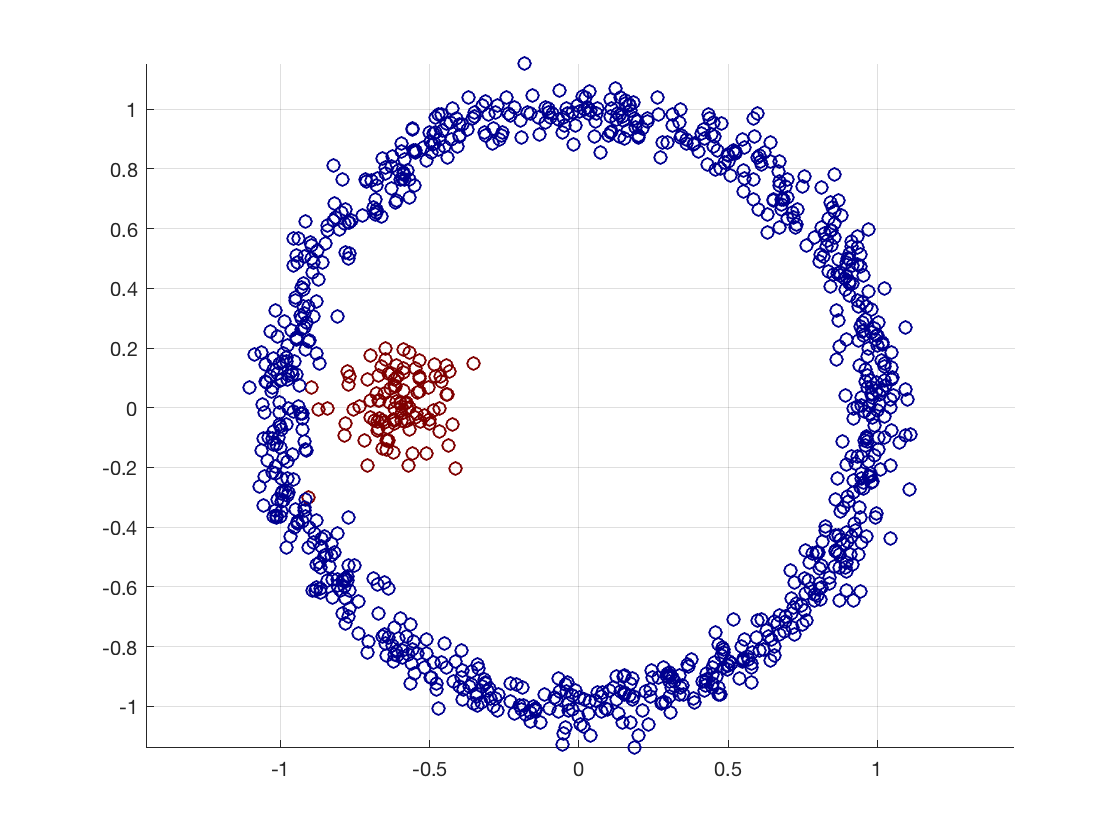
\includegraphics[width=0.4\linewidth]{hw4_4.png} ~~~
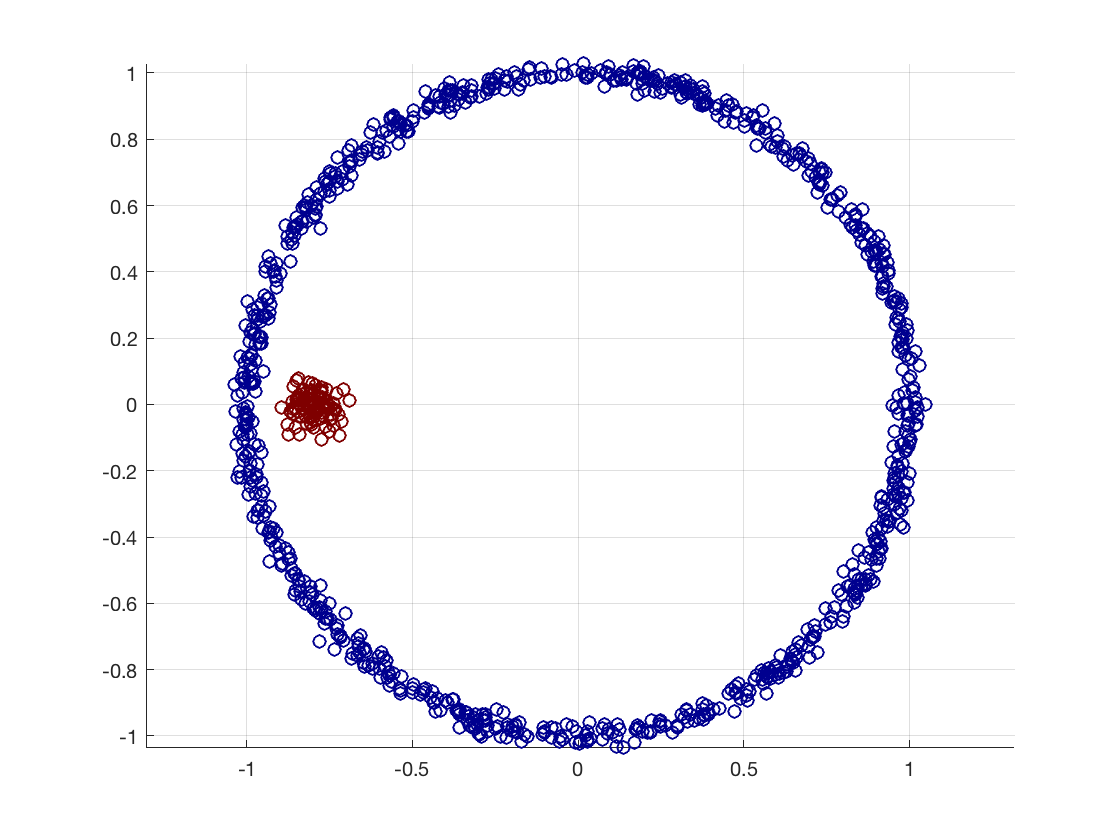
\includegraphics[width=0.4\linewidth]{hw4_3.png} 
}
\label{fig:1}
\end{figure}



\item
(Stochastic block model)
%
Consider the SBM where the graph has $n=100$ nodes, $k=4$ equal-size clusters, and $p_{ij}=0.8$ for $i,j$ in same cluster, and $p_{ij}=0.2$ otherwise.
A typical realization of the adjacency matrix $A$ is shown in the left of Figure \ref{fig:1}, 
where the matrix of $P$ is shown on the right, $A_{ij} \sim \text{Bern}(p_{ij})$.

\begin{figure}[h]
\centering{
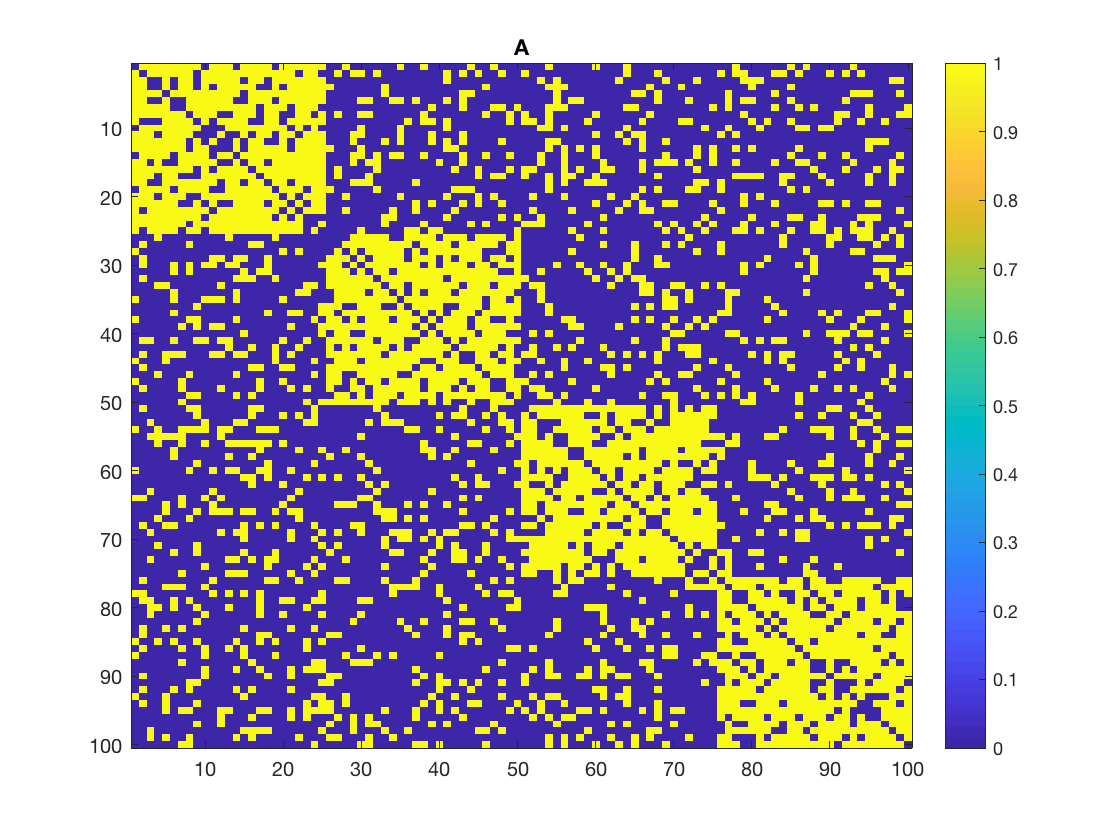
\includegraphics[width=0.4\linewidth]{hw4_1.png} ~~~
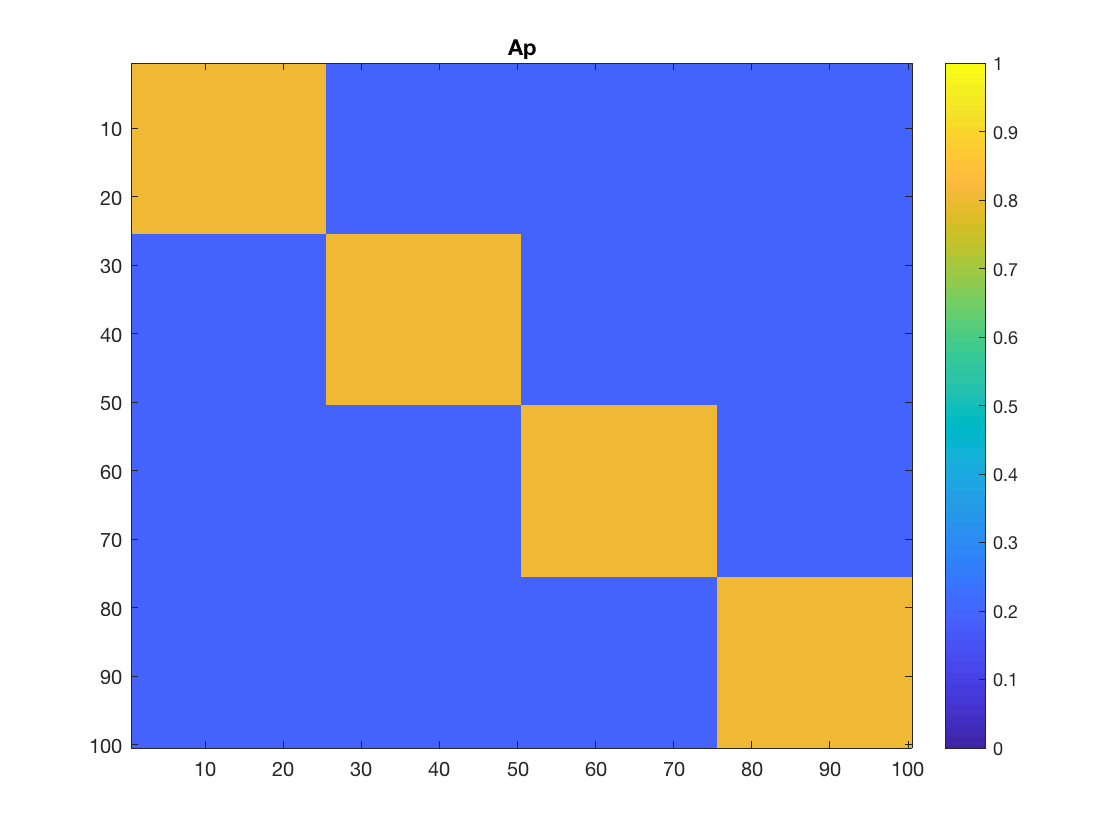
\includegraphics[width=0.4\linewidth]{hw4_2.png} 
}
\caption{
SBM with 4 blocks.
}
\label{fig:1}
\end{figure}


(1)
Effect of $n$ and $k$: what happens to the eigenvectors and eigenvalues of $A$ as $n$ increases? What if $k$ also increases? 

(2)
Effect of the balance of cluster size: what if cluster size is unequal?

(3) 
Effect of $B_{kl}$: what if $B_{kl} = p_{ij}$ for $i\in C_k$ and $j\in C_l$ are not necessarily constant across $k$ and $l$?

(4)
Effect of normalization: any difference in using $L_{\text{rw}}$, $L_{\text{sym}}$ or $L_{\text{un}}$? 



\end{enumerate}

\end{document}
